\documentclass[10pt,letterpaper]{article}\usepackage[]{graphicx}\usepackage[]{color}
%% maxwidth is the original width if it is less than linewidth
%% otherwise use linewidth (to make sure the graphics do not exceed the margin)
\makeatletter
\def\maxwidth{ %
  \ifdim\Gin@nat@width>\linewidth
    \linewidth
  \else
    \Gin@nat@width
  \fi
}
\makeatother

\definecolor{fgcolor}{rgb}{0.345, 0.345, 0.345}
\newcommand{\hlnum}[1]{\textcolor[rgb]{0.686,0.059,0.569}{#1}}%
\newcommand{\hlstr}[1]{\textcolor[rgb]{0.192,0.494,0.8}{#1}}%
\newcommand{\hlcom}[1]{\textcolor[rgb]{0.678,0.584,0.686}{\textit{#1}}}%
\newcommand{\hlopt}[1]{\textcolor[rgb]{0,0,0}{#1}}%
\newcommand{\hlstd}[1]{\textcolor[rgb]{0.345,0.345,0.345}{#1}}%
\newcommand{\hlkwa}[1]{\textcolor[rgb]{0.161,0.373,0.58}{\textbf{#1}}}%
\newcommand{\hlkwb}[1]{\textcolor[rgb]{0.69,0.353,0.396}{#1}}%
\newcommand{\hlkwc}[1]{\textcolor[rgb]{0.333,0.667,0.333}{#1}}%
\newcommand{\hlkwd}[1]{\textcolor[rgb]{0.737,0.353,0.396}{\textbf{#1}}}%

\usepackage{framed}
\makeatletter
\newenvironment{kframe}{%
 \def\at@end@of@kframe{}%
 \ifinner\ifhmode%
  \def\at@end@of@kframe{\end{minipage}}%
  \begin{minipage}{\columnwidth}%
 \fi\fi%
 \def\FrameCommand##1{\hskip\@totalleftmargin \hskip-\fboxsep
 \colorbox{shadecolor}{##1}\hskip-\fboxsep
     % There is no \\@totalrightmargin, so:
     \hskip-\linewidth \hskip-\@totalleftmargin \hskip\columnwidth}%
 \MakeFramed {\advance\hsize-\width
   \@totalleftmargin\z@ \linewidth\hsize
   \@setminipage}}%
 {\par\unskip\endMakeFramed%
 \at@end@of@kframe}
\makeatother

\definecolor{shadecolor}{rgb}{.97, .97, .97}
\definecolor{messagecolor}{rgb}{0, 0, 0}
\definecolor{warningcolor}{rgb}{1, 0, 1}
\definecolor{errorcolor}{rgb}{1, 0, 0}
\newenvironment{knitrout}{}{} % an empty environment to be redefined in TeX

\usepackage{alltt}
\usepackage[top=0.85in,left=2.75in,footskip=0.75in]{geometry}

% amsmath and amssymb packages, useful for mathematical formulas and symbols
\usepackage{amsmath,amssymb}

% Use adjustwidth environment to exceed column width (see example table in text)
\usepackage{changepage}

% Use Unicode characters when possible
\usepackage[utf8x]{inputenc}

% textcomp package and marvosym package for additional characters
\usepackage{textcomp,marvosym}

% cite package, to clean up citations in the main text. Do not remove.
\usepackage{cite}

% Use nameref to cite supporting information files (see Supporting Information section for more info)
\usepackage{nameref,hyperref}

% line numbers
\usepackage[right]{lineno}

% ligatures disabled
\usepackage{microtype}
\DisableLigatures[f]{encoding = *, family = * }

% color can be used to apply background shading to table cells only
\usepackage[table]{xcolor}

% array package and thick rules for tables
\usepackage{array}

% create "+" rule type for thick vertical lines
\newcolumntype{+}{!{\vrule width 2pt}}

% create \thickcline for thick horizontal lines of variable length
\newlength\savedwidth
\newcommand\thickcline[1]{%
  \noalign{\global\savedwidth\arrayrulewidth\global\arrayrulewidth 2pt}%
  \cline{#1}%
  \noalign{\vskip\arrayrulewidth}%
  \noalign{\global\arrayrulewidth\savedwidth}%
}

% \thickhline command for thick horizontal lines that span the table
\newcommand\thickhline{\noalign{\global\savedwidth\arrayrulewidth\global\arrayrulewidth 2pt}%
\hline
\noalign{\global\arrayrulewidth\savedwidth}}


% Remove comment for double spacing
%\usepackage{setspace} 
%\doublespacing

% Text layout
\raggedright
\setlength{\parindent}{0.5cm}
\textwidth 5.25in 
\textheight 8.75in

% Bold the 'Figure #' in the caption and separate it from the title/caption with a period
% Captions will be left justified
\usepackage[aboveskip=1pt,labelfont=bf,labelsep=period,justification=raggedright,singlelinecheck=off]{caption}
\renewcommand{\figurename}{Fig}

% Use the PLoS provided BiBTeX style
% \usepackage[backend=bibtex]{biblatex}
% \addbibresource{mybib.bib}

\bibliographystyle{plos2015}

% Remove brackets from numbering in List of References
\makeatletter
\renewcommand{\@biblabel}[1]{\quad#1.}
\makeatother

% Leave date blank
\date{}


% Header and Footer with logo
\usepackage{lastpage,fancyhdr,graphicx}
\usepackage{epstopdf}
\pagestyle{myheadings}
\pagestyle{fancy}
\fancyhf{}
\setlength{\headheight}{27.023pt}
\lhead{
\includegraphics[width=2.0in]{PLOS-submission.eps}}
\rfoot{\thepage/\pageref{LastPage}}
\renewcommand{\footrule}{\hrule height 2pt \vspace{2mm}}
\fancyheadoffset[L]{2.25in}
\fancyfootoffset[L]{2.25in}
\lfoot{\sf PLOS}

%% Include all macros below

\newcommand{\lorem}{{\bf LOREM}}
\newcommand{\ipsum}{{\bf IPSUM}}

%% END MACROS SECTION
\IfFileExists{upquote.sty}{\usepackage{upquote}}{}
\begin{document}
% \SweaveOpts{concordance=TRUE}
\vspace*{0.2in}
% Title must be 250 characters or less.
\begin{flushleft}
{\Large
\textbf\newline{A method for identifying households at high risk for mosquito borne illnesses.} % Please use "title case" (capitalize all terms in the title except conjunctions, prepositions, and articles).
}
\newline
% Insert author names, affiliations and corresponding author email (do not include titles, positions, or degrees).
\\
Dominic D. LaRoche\textsuperscript{1*},
Melanie L. Bell\textsuperscript{1},
Kacey C. Ernst\textsuperscript{1},
\\
\bigskip
\textbf{1} Mel & Enid Zuckerman College of Public Health, University of Arizona , Tucson, AZ, USA
\\
\bigskip

% Use the asterisk to denote corresponding authorship and provide email address in note below.
* dlaroche@email.arizona.edu

\end{flushleft}






% Please keep the abstract below 300 words
\section*{Abstract}
Mosquito borne illnesses are a significant threat to public health in countries where these diseases are either endemic or epidemic. Concerted efforts have been made in the past decade to reduce and in some cases eliminate mosquito borne diseases with the use of prophylactic interventions. The World Health Organization recommends preferential administration of interventions to those with the highest disease burden. However,  previous research has also identified the benefit of additionally targeting interventions at those with the highest risk of infections. We develop a methodology for identifying the highest risk households on landscape by combining both health risk and infection risk.  We use census information to determine health risk and we use a topographic wetness index to determine infection risk.  We implement the method to evaluate the administration of interventions at two sites in Kenya. We find preferential administration of interventions at the high-elevation epidemic-prone site but not at the low-elevation endemic site. Our results have important implications for assessing the administration of interventions in the battle against mosquito borne illnesses.

\linenumbers

\section*{Introduction}
%introduce the problem
Malaria and other mosquito borne illnesses are considered a significant threat to public health and a socio-economic burden in countries where these diseases are either endemic or epidemic \cite{Crouch}. Concerted efforts have been made in the past decade to reduce and in some cases eliminate malaria specifically. Many national strategic plans to reduce or eliminate malaria are in their third generation.  The World Health Organization recommends prioritizing the administration of interventions to pregnant women and young children followed by progressively achieving intervention coverage of all community members. The preferential administration of interventions to pregnant women and young children reflects the disproportionate disease burden borne by this group \cite{Bousema2012}. However,  previous research has identified the benefit of additionally targeting interventions at those with the highest risk of infections \cite{Schantz-Dunn2009}. Identifying individuals which are both vulnerable to infection and likely to be exposed to an infected mosquito is therefore a priority.  However, identifying high risk individuals can be costly and inefficient.\\

The Topographic Wetness Index (TWI) \cite{Beven1979} derived from freely available remotely-sensed topographic data has been previously investigated as a tool for assessing risk of malaria infection \cite{Cohen2008,Cohen2010}. TWI can potentially identify areas where water is likely to pool and Anopheles densities are likely to be higher. This method, therefore, has the potential to both inform new distribution campaigns and evaluate the efficacy of existing campaigns.  However, traditional TWI algorithms are complicated and generally require specialized software to implement.  Moreover, simply identifying areas where are mosquitoes are likely to breed does not account for the differential health risk of the exposed population.  We develop a simple, matrix-based, methodology using topographic data and combine this with a household census of demographics to identify high risk households.  We apply the method to two sites in Kenya where malaria is either endemic or epidemic-prone.  We compare our methodology to a traditional Topographic  Wetness Index by using knowledge of intervention use for two interventions at two sites in Kenya. \\%This method, therefore, has the potential to both inform new distribution campaigns and evaluate the efficacy of existing campaigns.



\section*{Materials and Methods}%main idea is to use traditional or aspect variance methods and see if there is a substantial difference.  Would be best 
Every household on a landscape will vary with respect to both the risk of exposure to mosquitoes and the number of at risk individuals in the household. We develop a method to combine these two risk factors into an overall risk score for each household within a management area in order to identify the households which will yield the greatest benefit from the application of limited resources.\\

\subsection{Topographical Wetness Index}

The Topographical Wetness index was originally introduced by Beven and Kirby in 1979 (\cite{Beven1979}).  TWI combines a measure of the amount of upstream drainage area with the local slope to determine the amount of wetness likely to accumulate at a point and is defined by Beven and Kirby generally as:
$$ln\frac{a}{tanb},$$
where $a$ is the local up-slope area (local area draining to the point) and $tanb$ is the local slope in radians.  The TWI is designed to predict the amount of water that is likely to flow into an area, based on surface topology, and the rate at which this water will flow out of an area.  Since TWI was first defined numerous methods have been developed to calculate it and several review papers have been published \cite{Quinn1995,Sørensen2006} as well as alternative modeling strategies developed \cite{Grabs2009}.  Areas with high in-flow and low out-flow are likely provide habitat for breeding mosquitoes. \\

The primary goal of using TWI in this application is to identify areas where mosquitoes are likely to breed.  However, the general TWI was originally designed to model surface water flow and not necessarily to identify areas where water will pool. A simpler algorithm for identifying only areas where water is likely to pool may perform as well, or better, than a general TWI algorithm and would not require specialized GIS software for implementation.  To examine this, we implement 2 different algorithms which differ in their calculation of the up-slope area and local slope: 1) the SAGA Wetness Index \cite{Bohner2002} (hereafter "general TWI"), and 2) a simplified topographic wetness index which simply identifies depressions without regard to up-slope area (hereafter "restricted TWI").  \\


We carried out all analyses using the statistical programming language R version 3.2.3 \cite{RCoreTeam2015}, with the exception of the SAGA TWI which was calculated with the SAGA open-source GIS software \cite{Bohner2006}.  Details for calculation of the general TWI are available in the software documentation available at \href{http://www.saga-gis.org/saga_module_doc/2.1.4/ta_hydrology.html}{ http://www.saga-gis.org\cite{Conrad2015}.  The method involves, for every point on the landscape:  calculating the up-slope area from which water will flow to the point,  calculating the catchment area, and the slope of the catchment area.  Areas with a larger up-slope area and a smaller catchment area slope are predicted to have more water accumulation.\\

In contrast to the relatively complicated calculation of a general TWI, we suggest a simple model based on identifying depressions with low outflow and disregarding the up-slope area.  We first identify depressions and valleys by identifying pixels which are lower than the average of their neighbors.  We do this by first calculating the average elevation of the surrounding pixels for each pixel ($p$) in the landscape at three resolutions of increasing size:  

$$\mu_{i,j} = \frac{\sum_{p \in j}e_p}{|p \in j|},$$

where $\mu_{i,j}$ is the average elevation of the pixels in the window of size $j$ surrounding pixel $i$.  The size of the windows is somewhat arbitrary but the idea is to identify small depressions from large ones so we suggest $90m \times 90m$, $210m \times 210m$, and $330m \times 330m$.  These sizes may be adjusted or tuned to a particular landscape if information is available to do so.  We then subtract the mean elevation from the actual elevation at each pixel from the three calculated averages and sum these differences.\\

$$\delta e_{i,j} = e_i - \mu_{i,j} $$
$$\Delta e_{i} = \sum_{j \in 1,2,3} \delta e_{i,j}$$

We then identify areas with low outflow by calculating the variance of the aspects (direction the slope faces) of neighboring pixels, $\theta$.  Since aspect is measured on a circular scale from 1 to 360 the variance of two aspects which are in fact quite close to each other but on opposite sides of the circular scale reset at 360 would be artificially high.  For example, the aspect of two points facing close to due north could be 359 and 1.  The variance of these two points would be $var(359,1)= 64082$.  However, the variance of two aspects of equal distance but not on opposite sides of the circular reset would be $var(1,3) = 2$.  In order to mitigate this difficulty we first translate each aspect to a cardinal direction denoted 1, 2, 3, or 4. We then calculate the variance of the aspects of the cells in each of 3 moving windows the same size as above ($90m \times 90m$, $210m \times 210m$, and $330m \times 330m$) and sum the resulting variances for each pixel:

$$\theta_{i} = \sum_{j \in 1,2,3} var(a_{i \in j}),$$

where $a_{i \in j}$ are the set of aspects in the moving window $j$  around pixel $i$.  The final wetness index is then calculated as, 
$$w_i = -1 \times \Delta e_i \times \theta_i.$$

Relatively large positive values of $w_i$ are expected to have higher wetness than small positive numbers.  Negative numbers indicate a ridge or peak and are therefore expected to be dry.\\
 

We assign each household a risk for exposure to mosquitoes (exposure risk hereafter) by deriving a continuous risk surface over the study area from each TWI algorithm.  We assume the mosquito exposure risk of a household is inversely related to the distance to one or more of these high-wetness areas.  Therefore,  we apply a Gaussian filter with $\sigma = 10$ to create a weighted average of mosquito risk for each cell in the study area.  The Gaussian filter is an isometric 2-dimensional smoothing function with a Gaussian kernel.  The value of $\sigma$ determines the degree of smoothing and should be scaled appropriately to match the resolution of the data.  The value of $\sigma$ can be tuned for a specific application if data is available and appropriate to do so. Each house is then assigned the risk score of the cell it is in or, for high resolution topographical data such as LiDAR (laser radar), the average of the cells a property occupies.\\


\subsection{Individual Health Risk}
Each household varied with respect to both the risk of exposure to mosquitoes and the number of at-risk individuals in the household. The household risk formulas will vary depending on the disease under study and the most vulnerable population(s) for that disease.  We recommend a simple additive risk score, like the score formula provided below developed for malaria, based on expert opinion or relevant literature. The sole purpose of the health risk score is to differentiate households with high risk from those with low risk.  More complicated formulas can be constructed but we believe a simple formula will be easier to interpret and adequate for most applications.\\

\subsection{Overall Risk}

To be at risk for a poor outcome a person must 1) come in contact with a disease harboring mosquito,  and 2) be inherently vulnerable to infection (e.g. very young or very old).  We create two risk scores representing each of these types of risk for every household on the landscape.  Since these risks will be calculated on different scales we center at 0 and standardize risk scores so that they are scale-independent.  These two scores can then be combined with a weighted sum to create an overall risk score for the household.  Weights in the sum are determined by expert opinion, in our example below we use equal weights.  This method lends itself well to the addition of additional risk scores, such as the distance to a health care provider, or even risk attenuating factors such as the presence of window screens, which can all be summed together with appropriate weights. 









\subsection{Example Analysis}

%Example Application
The government of Kenya developed the “National Malaria Strategy 2009-2017” in response to the ongoing threat of malaria \cite{Ministryofpublichealthandsanitation2009}. This strategy outlined 6 objectives,  the first of which is “to have at least 80\% of people living in malaria risk areas using appropriate malaria preventive interventions.” The two primary non-pharmaceutical interventions identified in the plan are Indoor Residual Spraying (IRS) and Long Lasting Insecticidal Nets (LLINs). The strategy outlined for achieving the intervention objective included the initial mass distribution of LLINs where malaria is either endemic (western lowlands) or epidemic-prone (western highlands); followed by routine distribution of LLINs to pregnant women and children under 1 year of age and a subsidized sale of LLINs. The strategy also outlined the use of widespread IRS followed by focal treatments in epidemic-prone areas, i.e. areas where mosquitoes are likely to breed.  We use this information to evaluate our methodology.\\

% The World Health Organization recommends prioritizing the administration of interventions to pregnant women and young children followed by progressively achieving intervention coverage of all community members. The preferential administration of interventions to pregnant women and young children reflects the disproportionate disease burden borne by this group \cite{Bousema2012}. However,  previous research has identified the benefit of additionally targeting interventions at those with the highest risk of infections \cite{Schantz-Dunn2009}. Identifying individuals which are both vulnerable to infection and likely to be exposed to an infected mosquito is therefore a priority.  However, existing distribution campaigns do not typically account for both infection risk and disease burden simultaneously.\\

Prior to the initiation of a community-based research program,  two study sites in western Kenya were mapped and a census was taken. These two sites represent the western highland (hereafter “epidemic-prone”,  N = 3380) and lowland (hereafter “endemic”,  N = 604) populations. Our objective was to determine if the highest risk households were given preference in the administration of interventions in the form of both bed nets and indoor residual spraying.\\

We collected demographic information for each occupant including age and sex. Both sites have had partial treatment with both LLINs and IRS and household heads provided initial information about LLIN ownership and government administration of household IRS in the previous six months.  We assigned an individual-based health risk score (health risk hereafter) to each household with the following formula:

$$Health\ Risk\ Score  =  (2 \times \ Children\ \leq 1) + (1 < \ Children\  \leq 5) + (2 \times \ Pregnant\ Women)$$

We assigned twice the weight to children under 1 and pregnant women since they have been previously identified as high risk \cite{Gupta1999, Snow1999, Menendez2000}.  This formula is tailored for malaria exposure but can be adjusted based on \emph{a priori} information about the individual risks for a particular mosquito borne disease. For example, for the Zika virus children may have a relatively low health risk whereas pregnant women and women of child bearing age may have much higher risk.\\

We added the standardized household health risk with the standardized household exposure risk to create a combined risk.  We then determined if high risk households are more likely to have received either a bed-net or aerial spraying with a logistic model;

$$log(\frac{p}{1-p}) = \beta_0 + \beta_1 \times \ Combined\ Household\ Risk, $$

where p  =  Probability of a house having a treatment.  If $e^{\beta_1}$ is $>$ 1 and statistically significant ($\alpha = 0.05$) then high-risk households are more likely to receive treatment.  %We used a restricted cubic spline function to determine if there was a linear relationship between the log odds of treatment and combined risk.  
We modeled the high and low sites separately because these sites differed substantially in topography and intervention administration protocols.  We also modeled the two interventions separately since they are administered under different protocols.  Finally, in order to examine the utility of each TWI algorithm, we repeated the analysis using both the general and restricted TWI.\\  %If we found evidence of a non-linear relationship we categorized the risk score into quartiles and re-fit with a means model. 




























\section*{Results}
The odds of receiving either a bed net or aerial spraying were higher for households with higher combined risk,  but only at the high site (Table~\ref{ORcmb}).  For each 1 standard deviation increase in combined risk at the high site the probability of receiving a bed net increased 27\% (OR: 1.27,  95\% CI: 1.18,  1.35) and the probability of aerial spraying increased 15\% (OR: 1.15,  95\% CI: 1.03,  1.29).  At the low site,  we found no preferential administration of either treatment to high combined risk households.  We found some evidence,  from the fitting of a restricted cubic spline,  of a non-linear relationship between the log-odds of net use and combined risk at the low site.  However,  accounting for non-linearity in the model did not change the results so we only report the linear model here.\\ 



\begin{table}[!ht]
\begin{adjustwidth}{-2.25in}{0in} % Comment out/remove adjustwidth environment if table fits in text column.
\centering
\caption{
{\bf Odds of receiving a treatment as a function of combined risk.} 
}
\begin{tabular}{lllll}
  \hline 
Site & Treatment & OR & Lower 95\% CI & Upper 95\% CI \\ 
  \hline
High & Net & 1.35 & 1.26 & 1.44 \\ 
   & Spray & 1.13 & 1.00 & 1.26 \\ 
  Low & Net & 1.09 & 0.86 & 1.39 \\ 
   & Spray & 0.9 & 0.61 & 1.34 \\ 
   \hline
\end{tabular}
\label{ORcmb}
\end{adjustwidth}
\end{table}

The probability of bed net use at the high site was more strongly associated with health risk,  whereas the probability of aerial spraying at the high site was more strongly associated with exposure risk (Table~\ref{ORtrt}).  However,  We did not find the same pattern at the low site where we found households with high exposure risk were actually significantly less likely to receive aerial spraying (OR: 0.35,  95\% CI: 0.14,  0.83).  \\






\begin{table}[!ht]
\caption{
{Odds of treatment from risk of either mosquito exposure or malaria risk.} 
}
\centering
\begin{tabular}{llllllll}
  \hline
 &  & \multicolumn{3}{l}{Health Risk} & \multicolumn{3}{l}{Exposure Risk}  \\ 
  
Site & Treatment & OR & Lower 95\% CI & Upper 95\% CI & OR & Lower 95\% CI & Upper 95\% CI \\ 
 \hline
  High & Net & 1.36 & 1.27 & 1.45 & 1.01 & 0.93 & 1.10 \\ 
   & Spray & 1.08 & 0.96 & 1.22 & 1.32 & 1.14 & 1.53 \\ 
  Low & Net & 1.21 & 0.94 & 1.55 & 0.58 & 0.31 & 1.10 \\ 
   & Spray & 1.08 & 0.67 & 1.74 & 0.34 & 0.15 & 0.79 \\ 
   \hline
\end{tabular}
\label{ORtrt}
\end{table}





















\subsection{Restricted TWI}

The use of the restricted TWI algorithm identified fewer regions as high risk than the general TWI at both sites and was less likely to assign exposure risk to areas near a channel (Fig~\ref{twis}).  The use of the restricted TWI based risk surface in the combined risk score increased the odds of a high-risk labelled household to have received a treatment for both the high and low sites,  although the increase in OR for the low site remained non-significant (Table~\ref{Sens}).

  


\begin{table}[!ht]
\begin{adjustwidth}{-2.25in}{0in} % Comment out/remove adjustwidth environment if table fits in text column.
\centering
\caption{
{\bf Comparison of results when constructing combined risk from the restricted TWI or general TWI.} 
}
\begin{tabular}{llllllll}
  \hline
 &  & \multicolumn{3}{l}{General TWI} & \multicolumn{3}{l}{Restricted TWI}\\
Site & Treatment & OR & Lower 95\% CI & Upper 95\% CI & OR & Lower 95\% CI & Upper 95\% CI \\ 
  \hline
High & Net & 1.35 & 1.26 & 1.44 & 1.45 & 1.33 & 1.59 \\ 
   & Spray & 1.13 & 1.00 & 1.26 & 1.22 & 1.05 & 1.42 \\ 
  Low & Net & 1.09 & 0.86 & 1.39 & 1.33 & 0.93 & 1.90 \\ 
   & Spray & 0.90 & 0.61 & 1.34 & 1.10 & 0.59 & 2.03 \\ 
   \hline
\end{tabular}
\label{Sens}
\end{adjustwidth}
\end{table}

\begin{figure}[!h]
\centering
% 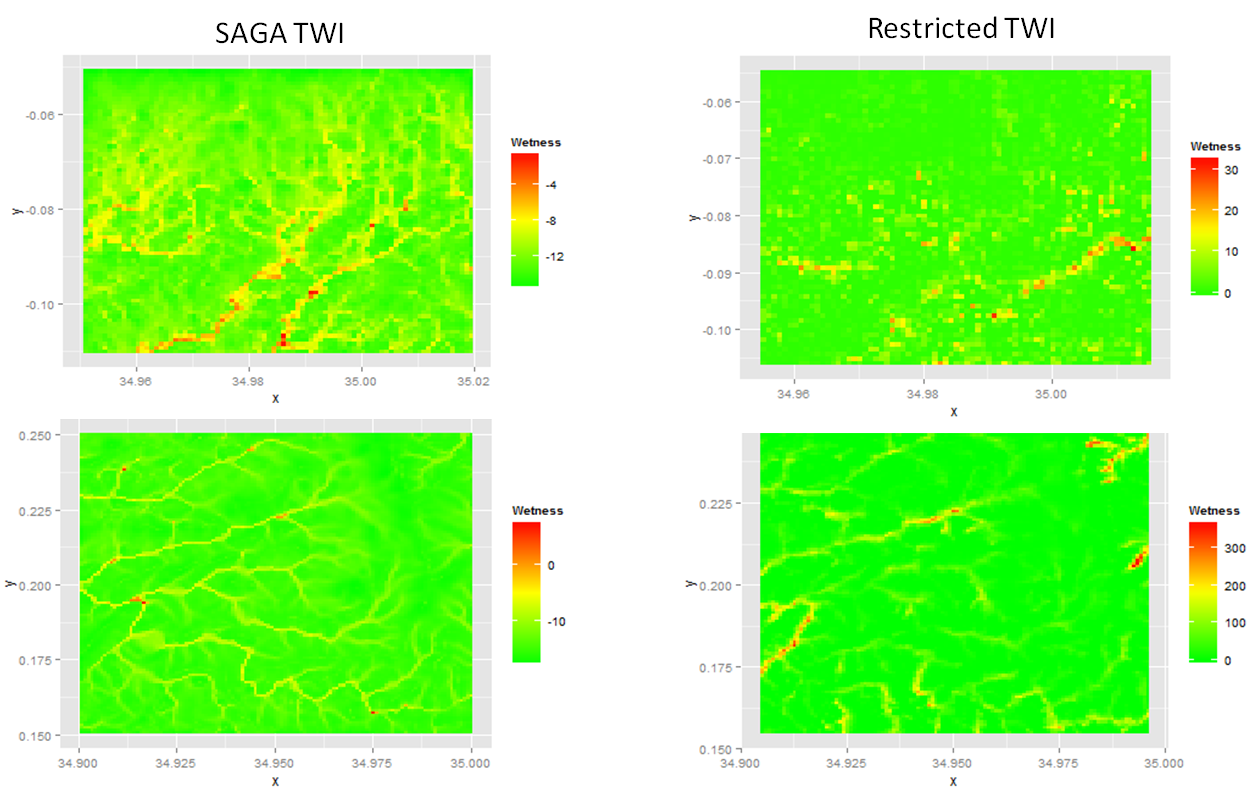
\includegraphics[scale=.5]{./figure/CompareTWI.png}
\caption{Comparison of the general TWI (left) and the restricted TWI (right) showing the lower extent of channels identified as moderate to high risk by the restricted TWI.  The restricted TWI also identified several areas missed by the general TWI. }
\label{twis}
\end{figure}



%Table 4.  Comparison of the odds of receiving a treatment based on health risk due to age with and without the inclusion of elderly household members. 


\section*{Discussion}
Our methodology is motivated by the need to improve the efficiency of intervention administration protocols and evaluate existing protocols.  Our example analysis evaluates existing protocols in which the administration of bed nets target pregnant women.  Therefore,  we would expect that households with young children would be more likely to have LLINs.  We found that health risk was associated with an increased probability of ILLN use at the high site but not the low site.  Similarly, under current protocols, aerial spraying is intended to target households at high risk for mosquito exposure  so we would expect that households with high exposure risk would be associated with aerial spraying.  Again,  this is the pattern we observed at the high site but not the low site where we found the opposite association.\\

Since we do not have mosquito incidence data we evaluate the efficacy of each TWI algorithm by how closely each algorithm matches our expectations based on the intervention administration protocol at each site.  The general TWI algorithm identified channels at both sites as moderate to high risk.  However, while these channels are likely to have higher wetness, the water may drain too quickly to provide quality breeding habitat for mosquitoes.  Use of the restricted TWI algorithm identified fewer channels as having moderate to high exposure risk while identifying some areas not identified by the general TWI algorithm (Fig~\ref{twis}).  Therefore, the restricted TWI algorithm may out-perform the general TWI in identifying mosquito breeding sites.  Our results comparing both TWI algorithms indicates a stronger association between the restricted TWI and intervention use indicating better alignment between the restricted TWI and mosquito risk assessments on the ground. This was particularly noticeable when evaluating the OR of a household receiving indoor residual spraying at the low site where the association was at least in the preferable direction, albeit not significantly.  We believe our method can be used to quickly evaluate the overall risk for a given household and improve the efficiency of distribution protocols.\\

Our method does not depend on accurately identifying the absolute risk of any given household, but rather the relative risk of every household on the landscape.  We believe the restricted TWI provides a simple and easily implemented algorithm for identifying high risk areas which may perform better than more complicated TWI algorithms based on the calculation of up-slope areas.  However, the sensitivity of our results to choice of TWI algorithm suggests that the TWI should be validated with additional information such as infection data.  This has been done previously (Cohen2008, Cohen2010),  but only with a single algorithm at a single site.  We recommend further evaluation of TWI algorithms with actual mosquito borne infection information at multiple sites, preferably with different topographies.\\


\nolinenumbers

\entry{Beven1979}{article}{}
  \name{author}{2}{}{%
    {{}%
     {BEVEN}{B.}%
     {K.~J.}{K.~J.}%
     {}{}%
     {}{}}%
    {{}%
     {KIRKBY}{K.}%
     {M.~J.}{M.~J.}%
     {}{}%
     {}{}}%
  }
  \list{language}{1}{%
    {en}%
  }
  \list{publisher}{1}{%
    {Taylor {\&} Francis Group}%
  }
  \strng{namehash}{BKJKMJ1}
  \strng{fullhash}{BKJKMJ1}
  \field{sortinit}{B}
  \field{abstract}{%
  Abstract A hydrological forecasting model is presented that attempts to
  combine the important distributed effects of channel network topology and
  dynamic contributing areas with the advantages of simple lumped parameter
  basin models. Quick response flow is predicted from a storage/contributing
  area relationship derived analytically from the topographic structure of a
  unit within a basin. Average soil water response is represented by a constant
  leakage infiltration store and an exponential subsurface water store. A
  simple non-linear routing procedure related to the link frequency
  distribution of the channel network completes the model and allows distinct
  basin sub-units, such as headwater and sideslope areas to be modelled
  separately. The model parameters are physically based in the sense that they
  may be determined directly by measurement and the model may be used at
  ungauged sites. Procedures for applying the model and tests with data from
  the Crimple Beck basin are described. Using only measured and est...%
  }
  \verb{doi}
  \verb 10.1080/02626667909491834
  \endverb
  \field{issn}{0303-6936}
  \field{number}{1}
  \field{pages}{43\bibrangedash 69}
  \field{title}{{A physically based, variable contributing area model of basin
  hydrology / Un mod{\`{e}}le {\`{a}} base physique de zone d'appel variable de
  l'hydrologie du bassin versant}}
  \verb{url}
  \verb http://www.tandfonline.com/doi/abs/10.1080/02626667909491834
  \endverb
  \field{volume}{24}
  \field{journaltitle}{Hydrological Sciences Bulletin}
  \field{year}{1979}
  \warn{\item Invalid format of field 'month'}
\endentry

\entry{Bohner2002}{misc}{}
  \name{author}{1}{}{%
    {{}%
     {B{\"{o}}hner}{B.}%
     {J}{J}%
     {}{}%
     {}{}}%
  }
  \list{publisher}{1}{%
    {The European Soil Bureau, Joint Research Centre}%
  }
  \strng{namehash}{BJ1}
  \strng{fullhash}{BJ1}
  \field{sortinit}{B}
  \field{booktitle}{Soil Classification 2001}
  \field{title}{{Soil Regionalisation by Means of Terrain Analysis and Process
  Parameterisation}}
  \list{location}{1}{%
    {Ispra}%
  }
  \field{year}{2002}
\endentry

\entry{Bohner2006}{article}{}
  \name{author}{2}{}{%
    {{}%
     {B{\"{o}}hner}{B.}%
     {J}{J}%
     {}{}%
     {}{}}%
    {{}%
     {Selige}{S.}%
     {T}{T}%
     {}{}%
     {}{}}%
  }
  \strng{namehash}{BJST1}
  \strng{fullhash}{BJST1}
  \field{sortinit}{B}
  \field{title}{{Spatial prediction of soil attributes using terrain analysis
  and climate regionalisation}}
  \verb{url}
  \verb http://www.pe.wzw.tum.de/publikationen/pdf/sd663.pdf
  \endverb
  \verb{file}
  \verb :C$\backslash$:/Users/dlaroche/AppData/Local/Mendeley Ltd./Mendeley Des
  \verb ktop/Downloaded/B{\"{o}}hner, Selige - 2006 - Spatial prediction of soi
  \verb l attributes using terrain analysis and climate regionalisation.pdf:pdf
  \endverb
  \field{journaltitle}{Gottinger Geographische Abhandlungen}
  \field{year}{2006}
\endentry

\entry{Bousema2012}{article}{}
  \name{author}{9}{}{%
    {{}%
     {Bousema}{B.}%
     {Teun}{T.}%
     {}{}%
     {}{}}%
    {{}%
     {Griffin}{G.}%
     {Jamie~T}{J.~T.}%
     {}{}%
     {}{}}%
    {{}%
     {Sauerwein}{S.}%
     {Robert~W}{R.~W.}%
     {}{}%
     {}{}}%
    {{}%
     {Smith}{S.}%
     {David~L}{D.~L.}%
     {}{}%
     {}{}}%
    {{}%
     {Churcher}{C.}%
     {Thomas~S}{T.~S.}%
     {}{}%
     {}{}}%
    {{}%
     {Takken}{T.}%
     {Willem}{W.}%
     {}{}%
     {}{}}%
    {{}%
     {Ghani}{G.}%
     {Azra}{A.}%
     {}{}%
     {}{}}%
    {{}%
     {Drakeley}{D.}%
     {Chris}{C.}%
     {}{}%
     {}{}}%
    {{}%
     {Gosling}{G.}%
     {Roly}{R.}%
     {}{}%
     {}{}}%
  }
  \list{publisher}{1}{%
    {Public Library of Science}%
  }
  \keyw{Disease Eradication,Humans,Malaria,Malaria: epidemiology,Malaria:
  prevention {\&} control,Malaria: transmission,Mosquito Control}
  \strng{namehash}{BT+1}
  \strng{fullhash}{BTGJTSRWSDLCTSTWGADCGR1}
  \field{sortinit}{B}
  \verb{doi}
  \verb 10.1371/journal.pmed.1001165
  \endverb
  \field{issn}{1549-1676}
  \field{number}{1}
  \field{pages}{e1001165}
  \field{title}{{Hitting hotspots: spatial targeting of malaria for control and
  elimination.}}
  \verb{url}
  \verb http://journals.plos.org/plosmedicine/article?id=10.1371/journal.pmed.1
  \verb 001165
  \endverb
  \field{volume}{9}
  \verb{file}
  \verb :C$\backslash$:/Users/dlaroche/AppData/Local/Mendeley Ltd./Mendeley Des
  \verb ktop/Downloaded/Bousema et al. - 2012 - Hitting hotspots spatial target
  \verb ing of malaria for control and elimination.pdf:pdf
  \endverb
  \field{journaltitle}{PLoS medicine}
  \field{year}{2012}
  \warn{\item Invalid format of field 'month'}
\endentry

\entry{Cohen2010}{article}{}
  \name{author}{6}{}{%
    {{}%
     {Cohen}{C.}%
     {Justin~M}{J.~M.}%
     {}{}%
     {}{}}%
    {{}%
     {Ernst}{E.}%
     {Kacey~C}{K.~C.}%
     {}{}%
     {}{}}%
    {{}%
     {Lindblade}{L.}%
     {Kim~A}{K.~A.}%
     {}{}%
     {}{}}%
    {{}%
     {Vulule}{V.}%
     {John~M}{J.~M.}%
     {}{}%
     {}{}}%
    {{}%
     {John}{J.}%
     {Chandy~C}{C.~C.}%
     {}{}%
     {}{}}%
    {{}%
     {Wilson}{W.}%
     {Mark~L}{M.~L.}%
     {}{}%
     {}{}}%
  }
  \keyw{Climate,Environment,Family
  Characteristics,Geography,Humans,Kenya,Kenya: epidemiology,Malaria,Malaria:
  epidemiology,Risk Factors,Water}
  \strng{namehash}{CJM+1}
  \strng{fullhash}{CJMEKCLKAVJMJCCWML1}
  \field{sortinit}{C}
  \field{abstract}{%
  BACKGROUND: Identification of high-risk malaria foci can help enhance
  surveillance or control activities in regions where they are most needed.
  Associations between malaria risk and land-use/land-cover are
  well-recognized, but these environmental characteristics are closely
  interrelated with the land's topography (e.g., hills, valleys, elevation),
  which also influences malaria risk strongly. Parsing the individual
  contributions of land-cover/land-use variables to malaria risk requires
  examining these associations in the context of their topographic landscape.
  This study examined whether environmental factors like land-cover, land-use,
  and urban density improved malaria risk prediction based solely on the
  topographically-determined context, as measured by the topographic wetness
  index. METHODS: The topographic wetness index, an estimate of predicted water
  accumulation in a defined area, was generated from a digital terrain model of
  the landscape surrounding households in two neighbouring western Kenyan
  highland communities. Variables determined to best encompass the variance in
  this topographic wetness surface were calculated at a household level.
  Land-cover/land-use information was extracted from a high-resolution
  satellite image using an object-based classification method. Topographic and
  land-cover variables were used individually and in combination to predict
  household-level malaria in the communities through an iterative split-sample
  model fitting and testing procedure. Models with only topographic variables
  were compared to those with additional predictive factors related to
  land-cover/land-use to investigate whether these environmental factors
  improved prediction of malaria based on the shape of the land alone. RESULTS:
  Variables related to topographic wetness proved most useful in predicting the
  households of individuals contracting malaria in this region of rugged
  terrain. Other variables related to human modification of the environment
  also demonstrated clear associations with household malaria. However, these
  land-cover/land-use variables failed to produce unambiguous improvements in
  statistical predictive models controlling for important topographic factors,
  with none improving prediction of household-level malaria more than 75{\%} of
  the time. CONCLUSIONS: Topographic wetness values in this region of highly
  varied terrain more accurately predicted houses at greater risk of malaria
  than did consideration of land-cover/land-use characteristics. As such, those
  planning control or local elimination strategies in similar highland regions
  may use topographic and geographic characteristics to effectively identify
  high-receptivity regions that may require enhanced vigilance.%
  }
  \verb{doi}
  \verb 10.1186/1475-2875-9-328
  \endverb
  \field{issn}{1475-2875}
  \field{pages}{328}
  \field{title}{{Local topographic wetness indices predict household malaria
  risk better than land-use and land-cover in the western Kenya highlands.}}
  \verb{url}
  \verb http://www.pubmedcentral.nih.gov/articlerender.fcgi?artid=2993734{\&}to
  \verb ol=pmcentrez{\&}rendertype=abstract
  \endverb
  \field{volume}{9}
  \verb{file}
  \verb :C$\backslash$:/Users/dlaroche/AppData/Local/Mendeley Ltd./Mendeley Des
  \verb ktop/Downloaded/Cohen et al. - 2010 - Local topographic wetness indices
  \verb  predict household malaria risk better than land-use and land-cover in
  \verb the wester.pdf:pdf
  \endverb
  \field{journaltitle}{Malaria journal}
  \field{year}{2010}
  \warn{\item Invalid format of field 'month'}
\endentry

\entry{Cohen2008}{article}{}
  \name{author}{6}{}{%
    {{}%
     {Cohen}{C.}%
     {Justin~M}{J.~M.}%
     {}{}%
     {}{}}%
    {{}%
     {Ernst}{E.}%
     {Kacey~C}{K.~C.}%
     {}{}%
     {}{}}%
    {{}%
     {Lindblade}{L.}%
     {Kim~A}{K.~A.}%
     {}{}%
     {}{}}%
    {{}%
     {Vulule}{V.}%
     {John~M}{J.~M.}%
     {}{}%
     {}{}}%
    {{}%
     {John}{J.}%
     {Chandy~C}{C.~C.}%
     {}{}%
     {}{}}%
    {{}%
     {Wilson}{W.}%
     {Mark~L}{M.~L.}%
     {}{}%
     {}{}}%
  }
  \list{language}{1}{%
    {En}%
  }
  \list{publisher}{1}{%
    {BioMed Central}%
  }
  \keyw{Altitude,Analysis of
  Variance,Animals,Housing,Humans,Humidity,Kenya,Kenya: epidemiology,Malaria,
  Falciparum,Malaria, Falciparum: epidemiology,Plasmodium falciparum,Residence
  Characteristics,Topography, Medical,Weather}
  \strng{namehash}{CJM+1}
  \strng{fullhash}{CJMEKCLKAVJMJCCWML1}
  \field{sortinit}{C}
  \field{abstract}{%
  BACKGROUND: Transmission of Plasmodium falciparum generally decreases with
  increasing elevation, in part because lower temperature slows the development
  of both parasites and mosquitoes. However, other aspects of the terrain, such
  as the shape of the land, may affect habitat suitability for Anopheles
  breeding and thus risk of malaria transmission. Understanding these local
  topographic effects may permit prediction of regions at high risk of malaria
  within the highlands at small spatial scales. METHODS: Hydrologic modelling
  techniques were adapted to predict the flow of water across the landscape
  surrounding households in two communities in the western Kenyan highlands.
  These surface analyses were used to generate indices describing predicted
  water accumulation in regions surrounding the study area. Households with and
  without malaria were compared for their proximity to regions of high and low
  predicted wetness. Predicted wetness and elevation variables were entered
  into bivariate and multivariate regression models to examine whether
  significant associations with malaria were observable at small spatial
  scales. RESULTS: On average, malaria case households (n = 423) were located
  280 m closer to regions with very high wetness indices than non-malaria
  "control" households (n = 895) (t = 10.35, p < 0.0001). Distance to high
  wetness indices remained an independent predictor of risk after controlling
  for household elevation in multivariate regression (OR = 0.93 [95{\%}
  confidence interval = 0.89-0.96] for a 100 m increase in distance). For every
  10 m increase in household elevation, there was a 12{\%} decrease in the odds
  of the house having a malaria case (OR = 0.88 [0.85-0.90]). However, after
  controlling for distance to regions of high predicted wetness and the
  community in which the house was located, this reduction in malaria risk was
  not statistically significant (OR = 0.98 [0.94-1.03]). CONCLUSION: Proximity
  to terrain with high predicted water accumulation was significantly and
  consistently associated with increased household-level malaria incidence,
  even at small spatial scales with little variation in elevation variables.
  These results suggest that high wetness indices are not merely proxies for
  valley bottoms, and hydrologic flow models may prove valuable for predicting
  areas of high malaria risk in highland regions. Application in areas where
  malaria surveillance is limited could identify households at higher risk and
  help focus interventions.%
  }
  \verb{doi}
  \verb 10.1186/1475-2875-7-40
  \endverb
  \field{issn}{1475-2875}
  \field{number}{1}
  \field{pages}{40}
  \field{title}{{Topography-derived wetness indices are associated with
  household-level malaria risk in two communities in the western Kenyan
  highlands.}}
  \verb{url}
  \verb http://malariajournal.biomedcentral.com/articles/10.1186/1475-2875-7-40
  \endverb
  \field{volume}{7}
  \verb{file}
  \verb :C$\backslash$:/Users/dlaroche/AppData/Local/Mendeley Ltd./Mendeley Des
  \verb ktop/Downloaded/Cohen et al. - 2008 - Topography-derived wetness indice
  \verb s are associated with household-level malaria risk in two communities i
  \verb n the west.pdf:pdf
  \endverb
  \field{journaltitle}{Malaria journal}
  \field{year}{2008}
  \warn{\item Invalid format of field 'month'}
\endentry

\entry{Crouch}{report}{}
  \name{author}{1}{}{%
    {{}%
     {Crouch}{C.}%
     {Margaret}{M.}%
     {}{}%
     {}{}}%
  }
  \strng{namehash}{CM1}
  \strng{fullhash}{CM1}
  \field{sortinit}{C}
  \field{title}{{The Second National Health Sector Strategic Plan of Kenya:
  NHSSP II – 2005–2010}}
  \verb{url}
  \verb http://www.healthpolicyinitiative.com/Publications/Documents/796{\_}1{\
  \verb _}796{\_}1{\_}NHSSP{\_}II.pdf
  \endverb
  \list{institution}{1}{%
    {Republic of Kenya Ministry of Health}%
  }
  \field{type}{techreport}
\endentry

\entry{Grabs2009}{article}{}
  \name{author}{4}{}{%
    {{}%
     {Grabs}{G.}%
     {T.}{T.}%
     {}{}%
     {}{}}%
    {{}%
     {Seibert}{S.}%
     {J.}{J.}%
     {}{}%
     {}{}}%
    {{}%
     {Bishop}{B.}%
     {K.}{K.}%
     {}{}%
     {}{}}%
    {{}%
     {Laudon}{L.}%
     {H.}{H.}%
     {}{}%
     {}{}}%
  }
  \keyw{Distributed hydrological model,Landscape analysis,Saturated
  areas,Spatial patterns,Topographic wetness index,Wetlands}
  \strng{namehash}{GT+1}
  \strng{fullhash}{GTSJBKLH1}
  \field{sortinit}{G}
  \field{abstract}{%
  Topography is often one of the major controls on the spatial pattern of
  saturated areas, which in turn is a key to understanding much of the
  variability in soils, hydrological processes, and stream water quality. The
  topographic wetness index (TWI) has become a widely used tool to describe
  wetness conditions at the catchment scale. With this index, however, it is
  assumed that groundwater gradients always equal surface gradients. To
  overcome this limitation, we suggest deriving wetness indices based on
  simulations of distributed catchment models. We compared these new indices
  with the TWI and evaluated the different indices by their capacity to predict
  spatial patterns of saturated areas. Results showed that the model-derived
  wetness indices predicted the spatial distribution of wetlands significantly
  better than the TWI. These results encourage the use of a dynamic distributed
  hydrological model to derive wetness index maps for hydrological landscape
  analysis in catchments with topographically driven groundwater tables.%
  }
  \verb{doi}
  \verb 10.1016/j.jhydrol.2009.03.031
  \endverb
  \field{issn}{00221694}
  \field{number}{1-2}
  \field{pages}{15\bibrangedash 23}
  \field{title}{{Modeling spatial patterns of saturated areas: A comparison of
  the topographic wetness index and a dynamic distributed model}}
  \verb{url}
  \verb http://www.sciencedirect.com/science/article/pii/S002216940900211X
  \endverb
  \field{volume}{373}
  \field{journaltitle}{Journal of Hydrology}
  \field{year}{2009}
  \warn{\item Invalid format of field 'month'}
\endentry

\entry{Gupta1999}{article}{}
  \name{author}{5}{}{%
    {{}%
     {Gupta}{G.}%
     {S}{S}%
     {}{}%
     {}{}}%
    {{}%
     {Snow}{S.}%
     {R~W}{R.~W.}%
     {}{}%
     {}{}}%
    {{}%
     {Donnelly}{D.}%
     {C~A}{C.~A.}%
     {}{}%
     {}{}}%
    {{}%
     {Marsh}{M.}%
     {K}{K}%
     {}{}%
     {}{}}%
    {{}%
     {Newbold}{N.}%
     {C}{C}%
     {}{}%
     {}{}}%
  }
  \keyw{Africa South of the Sahara,Africa South of the Sahara:
  epidemiology,Child,Child, Preschool,Humans,Infant,Malaria,
  Falciparum,Malaria, Falciparum: epidemiology,Malaria, Falciparum: immunology}
  \strng{namehash}{GS+1}
  \strng{fullhash}{GSSRWDCAMKNC1}
  \field{sortinit}{G}
  \field{abstract}{%
  In areas of stable transmission, clinical immunity to mild malaria is
  acquired slowly, so it is not usually effective until early adolescence.
  Life-threatening disease is, however, restricted to a much younger age group,
  indicating that resistance to the severe clinical consequences of infection
  is acquired more quickly. Understanding how rapidly immunity develops to
  severe malaria is essential, as severe malaria should be the primary target
  of intervention strategies, and predicting the result of interventions that
  reduce host exposure will require consideration of these dynamics. Severe
  disease in childhood is less frequent in areas where transmission is the
  greatest. One explanation for this is that infants experience increased
  exposure to infection while they are protected from disease, possibly by
  maternal antibody. They therefore emerge from this period of clinical
  protection with considerably more immunity than those who experience lower
  transmission intensities. Here we use this data, assuming a period of
  clinical protection, to estimate the number of prior infections needed to
  reduce the risk of severe disease to negligible levels. Contrary to
  expectations, one or two successful infective bites seem to be all that is
  necessary across a broad range of transmission intensities.%
  }
  \verb{doi}
  \verb 10.1038/6560
  \endverb
  \field{issn}{1078-8956}
  \field{number}{3}
  \field{pages}{340\bibrangedash 3}
  \field{title}{{Immunity to non-cerebral severe malaria is acquired after one
  or two infections.}}
  \verb{url}
  \verb http://www.ncbi.nlm.nih.gov/pubmed/10086393
  \endverb
  \field{volume}{5}
  \field{journaltitle}{Nature medicine}
  \field{year}{1999}
  \warn{\item Invalid format of field 'month'}
\endentry

\entry{Ministryofpublichealthandsanitation2009}{report}{}
  \name{author}{2}{}{%
    {{}%
     {health}{h.}%
     {Ministry}{M.}%
     {of~public}{o.~p.}%
     {}{}}%
    {{}%
     {sanitation}{s.}%
     {}{}%
     {}{}%
     {}{}}%
  }
  \strng{namehash}{hMops1}
  \strng{fullhash}{hMops1}
  \field{sortinit}{H}
  \field{number}{July}
  \field{pages}{116}
  \field{title}{{National Malaria Strategy 2009-2017}}
  \verb{url}
  \verb https://www.google.com/url?sa=t{\&}rct=j{\&}q={\&}esrc=s{\&}source=web{
  \verb \&}cd=1{\&}ved=0CB4QFjAAahUKEwiXj76j-IzHAhWGVT4KHZD7AFA{\&}url=http://w
  \verb ww.c-hubonline.org/sites/default/files/resources/main/Kenya{\_}National
  \verb {\_}Malaria{\_}Strategy{\_}2009-2017.pdf{\&}ei=9GG{\_}VZfFKIar-QGQ94OAB
  \verb Q{\&}usg=AFQj
  \endverb
  \list{institution}{2}{%
    {Ministry of public health}%
    {sanitation}%
  }
  \field{type}{techreport}
  \field{year}{2009}
\endentry

\entry{Menendez2000}{article}{}
  \name{author}{3}{}{%
    {{}%
     {Menendez}{M.}%
     {C}{C}%
     {}{}%
     {}{}}%
    {{}%
     {Fleming}{F.}%
     {A~F}{A.~F.}%
     {}{}%
     {}{}}%
    {{}%
     {Alonso}{A.}%
     {P~L}{P.~L.}%
     {}{}%
     {}{}}%
  }
  \keyw{Adult,Anemia,Anemia: etiology,Antimalarials,Antimalarials: therapeutic
  use,Child,Erythrocytes,Erythrocytes: drug
  effects,Female,Hemolysis,Humans,Malaria, Falciparum,Malaria, Falciparum:
  complications,Malaria, Falciparum: drug therapy,Male,Pregnancy,Pregnancy
  Complications, Parasitic}
  \strng{namehash}{MCFAFAPL1}
  \strng{fullhash}{MCFAFAPL1}
  \field{sortinit}{M}
  \field{abstract}{%
  Malaria infection in humans by Plasmodium species is associated with a
  reduction in haemoglobin levels, frequently leading to anaemia. Plasmodium
  falciparum causes the most severe and profound anaemia, with a significant
  risk of death. This cannot be explained simply by the direct destruction of
  parasitized red blood cells at the time of release of merozoites, a process
  shared by all these species. In this review, Clara Menendez, Alan Fleming and
  Pedro Alonso focus on recent advances in our knowledge of the
  pathophysiology, epidemiology, management and prevention of anaemia from
  falciparum malaria.%
  }
  \field{issn}{0169-4758}
  \field{number}{11}
  \field{pages}{469\bibrangedash 76}
  \field{title}{{Malaria-related anaemia.}}
  \verb{url}
  \verb http://www.ncbi.nlm.nih.gov/pubmed/11063857
  \endverb
  \field{volume}{16}
  \field{journaltitle}{Parasitology today (Personal ed.)}
  \field{year}{2000}
  \warn{\item Invalid format of field 'month'}
\endentry

\entry{Quinn1995}{article}{}
  \name{author}{3}{}{%
    {{}%
     {Quinn}{Q.}%
     {P.~F.}{P.~F.}%
     {}{}%
     {}{}}%
    {{}%
     {Beven}{B.}%
     {K.~J.}{K.~J.}%
     {}{}%
     {}{}}%
    {{}%
     {Lamb}{L.}%
     {R.}{R.}%
     {}{}%
     {}{}}%
  }
  \strng{namehash}{QPFBKJLR1}
  \strng{fullhash}{QPFBKJLR1}
  \field{sortinit}{Q}
  \verb{doi}
  \verb 10.1002/hyp.3360090204
  \endverb
  \field{issn}{08856087}
  \field{number}{2}
  \field{pages}{161\bibrangedash 182}
  \field{title}{{The in(a/tan/$\beta$) index: How to calculate it and how to
  use it within the topmodel framework}}
  \verb{url}
  \verb http://doi.wiley.com/10.1002/hyp.3360090204
  \endverb
  \field{volume}{9}
  \field{journaltitle}{Hydrological Processes}
  \field{year}{1995}
  \warn{\item Invalid format of field 'month'}
\endentry

\entry{RCoreTeam2015}{misc}{}
  \name{author}{1}{}{%
    {{}%
     {{R Core Team}}{R.}%
     {}{}%
     {}{}%
     {}{}}%
  }
  \list{publisher}{1}{%
    {R Foundation for Statistical Computing}%
  }
  \strng{namehash}{R1}
  \strng{fullhash}{R1}
  \field{sortinit}{R}
  \field{title}{{R: A Language and Environment for Statistical Computing}}
  \verb{url}
  \verb https://www.r-project.org/
  \endverb
  \list{location}{1}{%
    {Vienna, Austria}%
  }
  \field{year}{2015}
\endentry

\entry{Schantz-Dunn2009}{article}{}
  \name{author}{2}{}{%
    {{}%
     {Schantz-Dunn}{S.-D.}%
     {Julianna}{J.}%
     {}{}%
     {}{}}%
    {{}%
     {Nour}{N.}%
     {Nawal~M}{N.~M.}%
     {}{}%
     {}{}}%
  }
  \strng{namehash}{SDJNNM1}
  \strng{fullhash}{SDJNNM1}
  \field{sortinit}{S}
  \field{abstract}{%
  Malaria, a parasitic infection transmitted by mosquitoes, is one of the most
  devastating infectious diseases, killing more than 1 million people annually.
  Pregnant women, children, and immunocompromised individuals have the highest
  morbidity and mortality, and Africa bears the heaviest burden. The World
  Health Organization defines malaria as a disease of poverty caused by
  poverty. Pregnant women infected with malaria usually have more severe
  symptoms and outcomes, with higher rates of miscarriage, intrauterine demise,
  premature delivery, low-birth-weight neonates, and neonatal death. They are
  also at a higher risk for severe anemia and maternal death. Malaria can be
  prevented with appropriate drugs, bed nets treated with insecticide, and
  effective educational outreach programs.%
  }
  \field{issn}{1941-2797}
  \field{number}{3}
  \field{pages}{186\bibrangedash 92}
  \field{title}{{Malaria and pregnancy: a global health perspective.}}
  \verb{url}
  \verb http://www.pubmedcentral.nih.gov/articlerender.fcgi?artid=2760896{\&}to
  \verb ol=pmcentrez{\&}rendertype=abstract
  \endverb
  \field{volume}{2}
  \verb{file}
  \verb :C$\backslash$:/Users/dlaroche/AppData/Local/Mendeley Ltd./Mendeley Des
  \verb ktop/Downloaded/Schantz-Dunn, Nour - 2009 - Malaria and pregnancy a glo
  \verb bal health perspective.pdf:pdf
  \endverb
  \field{journaltitle}{Reviews in obstetrics {\&} gynecology}
  \field{year}{2009}
  \warn{\item Invalid format of field 'month'}
\endentry

\entry{Snow1999}{article}{}
  \name{author}{4}{}{%
    {{}%
     {Snow}{S.}%
     {R~W}{R.~W.}%
     {}{}%
     {}{}}%
    {{}%
     {Craig}{C.}%
     {M}{M}%
     {}{}%
     {}{}}%
    {{}%
     {Deichmann}{D.}%
     {U}{U}%
     {}{}%
     {}{}}%
    {{}%
     {Marsh}{M.}%
     {K}{K}%
     {}{}%
     {}{}}%
  }
  \keyw{Adolescent,Adult,Africa,Africa South of the Sahara,Africa South of the
  Sahara: epidemiology,Africa, Northern,Africa, Northern: epidemiology,Africa:
  epidemiology,Age Factors,Anemia,Anemia: etiology,Blood Transfusion,Blood
  Transfusion: adverse effects,Child,Child, Preschool,Climate,Disabled
  Children,Female,HIV Infections,HIV Infections: etiology,Humans,Infant,Infant,
  Newborn,Malaria,Malaria, Cerebral,Malaria, Cerebral: complications,Malaria,
  Cerebral: epidemiology,Malaria, Cerebral: mortality,Malaria,
  Falciparum,Malaria, Falciparum: epidemiology,Malaria, Falciparum:
  mortality,Malaria: complications,Malaria: epidemiology,Malaria:
  mortality,Male,Risk Factors}
  \strng{namehash}{SRW+1}
  \strng{fullhash}{SRWCMDUMK1}
  \field{sortinit}{S}
  \field{abstract}{%
  The contribution of malaria to morbidity and mortality among people in Africa
  has been a subject of academic interest, political advocacy, and speculation.
  National statistics for much of sub-Saharan Africa have proved to be an
  unreliable source of disease-specific morbidity and mortality data. Credible
  estimates of disease-specific burdens are required for setting global and
  national priorities for health in order to rationalize the use of limited
  resources and lobby for financial support. We have taken an empirical
  approach to defining the limits of Plasmodium falciparum transmission across
  the continent and interpolated the distributions of projected populations in
  1995. By combining a review of the literature on malaria in Africa and models
  of acquired functional immunity, we have estimated the age-structured rates
  of the fatal, morbid and disabling sequelae following exposure to malaria
  infection under different epidemiological conditions. This research seeks to
  estimate mortality, morbidity, and disability due to malaria among Africa's
  nonpregnant population. It uses an empirical approach to define Plasmodium
  falciparum transmission limits across the continent. And, the distributions
  of projected populations in 1995 are interjected. The review of literature on
  malaria in Africa and models of acquired functional immunity served as a
  basis for the researchers to predict the age-structured rates of the fatal,
  morbid and disabling consequences following malaria infection. These
  estimates were tabulated and analyzed. The results indicated that among
  populations exposed to stable endemic malaria in sub-Saharan Africa,
  approximately 987,466 people might have died in 1995 due to malaria
  infection. On the other hand, over 207.5 million clinical attacks of malaria
  may have occurred.%
  }
  \field{issn}{0042-9686}
  \field{number}{8}
  \field{pages}{624\bibrangedash 40}
  \field{title}{{Estimating mortality, morbidity and disability due to malaria
  among Africa's non-pregnant population.}}
  \verb{url}
  \verb http://www.pubmedcentral.nih.gov/articlerender.fcgi?artid=2557714{\&}to
  \verb ol=pmcentrez{\&}rendertype=abstract
  \endverb
  \field{volume}{77}
  \verb{file}
  \verb :C$\backslash$:/Users/dlaroche/AppData/Local/Mendeley Ltd./Mendeley Des
  \verb ktop/Downloaded/Snow et al. - 1999 - Estimating mortality, morbidity an
  \verb d disability due to malaria among Africa's non-pregnant population.pdf:
  \verb pdf
  \endverb
  \field{journaltitle}{Bulletin of the World Health Organization}
  \field{year}{1999}
  \warn{\item Invalid format of field 'month'}
\endentry

\entry{Sørensen2006}{article}{}
  \name{author}{3}{}{%
    {{}%
     {S{\o}rensen}{S.}%
     {R.}{R.}%
     {}{}%
     {}{}}%
    {{}%
     {Zinko}{Z.}%
     {U.}{U.}%
     {}{}%
     {}{}}%
    {{}%
     {Seibert}{S.}%
     {J.}{J.}%
     {}{}%
     {}{}}%
  }
  \list{language}{1}{%
    {English}%
  }
  \list{publisher}{1}{%
    {Copernicus GmbH}%
  }
  \strng{namehash}{SRZUSJ1}
  \strng{fullhash}{SRZUSJ1}
  \field{sortinit}{S}
  \verb{doi}
  \verb 10.5194/hess-10-101-2006
  \endverb
  \field{issn}{1607-7938}
  \field{number}{1}
  \field{pages}{101\bibrangedash 112}
  \field{title}{{On the calculation of the topographic wetness index:
  evaluation of different methods based on field observations}}
  \verb{url}
  \verb http://www.hydrol-earth-syst-sci.net/10/101/2006/hess-10-101-2006.html
  \endverb
  \field{volume}{10}
  \verb{file}
  \verb :C$\backslash$:/Users/dlaroche/AppData/Local/Mendeley Ltd./Mendeley Des
  \verb ktop/Downloaded/S{\o}rensen, Zinko, Seibert - 2006 - On the calculation
  \verb  of the topographic wetness index evaluation of different methods based
  \verb  on field obs.pdf:pdf
  \endverb
  \field{journaltitle}{Hydrology and Earth System Sciences}
  \field{year}{2006}
  \warn{\item Invalid format of field 'month'}
\endentry



\end{document}
